\section{Experiments}
\label{sec:exp}

Our experiments ask four questions. RQ1: does repairing the scorer improve OPD across teachers, students and environments? RQ2: can the takeovers be selected without reward? RQ3: which parts of \method{} are necessary? RQ4: what does the repaired scorer change in long-horizon behavior? We answer these questions below.

\begin{table}[t]
\centering
\caption{\textbf{Main results: \method{} versus vanilla OPD, TCOD-F2B, Guided-OPD and FutureBridge.} Success (\%) of one training run per cell, mean$\pm$std over three decodes of its final checkpoint; every split in \Cref{tab:main-full}. The \colorbox{box_green!12}{\textcolor{box_green}{best}} and \colorbox{box_red!12}{\textcolor{box_red}{second best}} of the five trained students in each column are highlighted.}
\label{tab:main}
\small
\setlength{\tabcolsep}{4.5pt}
\begin{tabular}{@{}lcccccc@{}}
\toprule
\multirow{3}{*}{Method} & \multicolumn{6}{c}{Qwen3.5-9B $\to$ Qwen3.5-2B\,/\,4B} \\
\cmidrule(lr){2-7}
 & \multicolumn{2}{c}{ALFWorld} & \multicolumn{2}{c}{WebShop} & \multicolumn{2}{c}{ScienceWorld} \\
\cmidrule(lr){2-3}\cmidrule(lr){4-5}\cmidrule(lr){6-7}
 & 2B & 4B & 2B & 4B & 2B & 4B \\
\midrule\midrule
Teacher alone & \multicolumn{2}{c}{$63.1{\pm}1.7$} & \multicolumn{2}{c}{$33.5{\pm}0.3$} & \multicolumn{2}{c}{$32.0{\pm}1.8$} \\
Student alone & $15.1{\pm}1.8$ & $43.4{\pm}1.0$ & $17.6{\pm}1.1$ & $33.7{\pm}0.9$ & $3.1{\pm}0.4$ & $28.0{\pm}1.5$ \\
\midrule
Vanilla OPD & $58.0{\pm}2.4$ & \secondscore{$65.8{\pm}2.6$} & $35.7{\pm}1.6$ & $34.6{\pm}2.9$ & $23.7{\pm}2.0$ & \secondscore{$34.6{\pm}3.5$} \\
TCOD-F2B & $62.7{\pm}2.0$ & $59.6{\pm}1.5$ & $33.1{\pm}0.5$ & $35.1{\pm}0.9$ & \secondscore{$28.0{\pm}2.6$} & $30.6{\pm}0.7$ \\
Guided-OPD & \secondscore{$63.6{\pm}2.2$} & $61.6{\pm}2.0$ & $35.6{\pm}0.6$ & \secondscore{$35.5{\pm}1.3$} & $25.9{\pm}3.7$ & $32.2{\pm}1.1$ \\
FutureBridge & $56.8{\pm}2.8$ & $58.4{\pm}3.7$ & \secondscore{$36.3{\pm}1.0$} & $33.9{\pm}1.7$ & $19.0{\pm}2.0$ & $30.7{\pm}1.3$ \\
\textbf{\textcolor{box_green}{\method{} (ours)}} & \bestscore{$77.9{\pm}1.3$} & \bestscore{$81.9{\pm}2.4$} & \bestscore{$57.9{\pm}1.6$} & \bestscore{$55.9{\pm}1.4$} & \bestscore{$37.9{\pm}0.6$} & \bestscore{$47.8{\pm}3.0$} \\
\midrule[\heavyrulewidth]
\multirow{3}{*}{Method} & \multicolumn{6}{c}{Qwen3-30B-A3B-Instruct-2507 $\to$ Qwen3-4B\,/\,8B} \\
\cmidrule(lr){2-7}
 & \multicolumn{2}{c}{ALFWorld} & \multicolumn{2}{c}{WebShop} & \multicolumn{2}{c}{ScienceWorld} \\
\cmidrule(lr){2-3}\cmidrule(lr){4-5}\cmidrule(lr){6-7}
 & 4B & 8B & 4B & 8B & 4B & 8B \\
\midrule\midrule
Teacher alone & \multicolumn{2}{c}{$42.3{\pm}1.1$} & \multicolumn{2}{c}{$2.9{\pm}0.3$} & \multicolumn{2}{c}{$32.9{\pm}3.2$} \\
Student alone & $30.4{\pm}2.3$ & $46.9{\pm}0.8$ & $15.5{\pm}1.2$ & $23.6{\pm}1.2$ & $9.0{\pm}1.4$ & $24.0{\pm}3.9$ \\
\midrule
Vanilla OPD & $41.2{\pm}1.7$ & $44.5{\pm}2.6$ & \secondscore{$24.7{\pm}1.1$} & $20.3{\pm}0.9$ & $38.0{\pm}1.2$ & $36.8{\pm}1.0$ \\
TCOD-F2B & \secondscore{$42.6{\pm}1.1$} & \secondscore{$48.8{\pm}1.8$} & $22.8{\pm}0.7$ & \secondscore{$23.4{\pm}0.7$} & \secondscore{$38.4{\pm}0.9$} & $34.9{\pm}0.5$ \\
Guided-OPD & $42.0{\pm}0.4$ & $47.0{\pm}1.9$ & $23.3{\pm}1.6$ & $22.3{\pm}0.8$ & $34.7{\pm}1.8$ & $33.0{\pm}1.5$ \\
FutureBridge & $41.8{\pm}2.6$ & $45.9{\pm}1.1$ & $16.7{\pm}0.9$ & $20.7{\pm}0.7$ & $36.1{\pm}1.5$ & \secondscore{$37.1{\pm}2.0$} \\
\textbf{\textcolor{box_green}{\method{} (ours)}} & \bestscore{$54.5{\pm}1.4$} & \bestscore{$54.7{\pm}1.0$} & \bestscore{$28.5{\pm}0.6$} & \bestscore{$30.4{\pm}1.2$} & \bestscore{$45.8{\pm}1.4$} & \bestscore{$50.5{\pm}1.4$} \\
\bottomrule
\end{tabular}
\end{table}


\subsection{Setup}
\label{sec:exp-setup}

\textbf{Teachers and students.}
Qwen3.5-9B~\citep{qwen352026} teaches Qwen3.5-2B and Qwen3.5-4B on three environments, and Qwen3.5-4B teaches itself in \Cref{tab:self}.
Qwen3-30B-A3B-Instruct-2507~\citep{qwen32025} teaches Qwen3-4B and Qwen3-8B on the same three environments.
We chose these pairs to vary three things: model size, from 2B to 30B parameters; model generation, Qwen3.5 and Qwen3; and architecture, a dense 9B teacher and a mixture-of-experts 30B-A3B teacher.
Every prompt carries one fixed worked demonstration per environment; native reasoning mode is off, and each turn opens with one to three sentences of plain-text deliberation before the tool call, as detailed in \Cref{app:protocol}.

\textbf{Environments.}
ALFWorld (household tasks), WebShop (shopping) and ScienceWorld (science experiments) are scored by success (\%). ALFWorld and ScienceWorld have a seen and an unseen split, and the main text reports their mean; WebShop is evaluated on its 500 canonical goals. Following TCOD, the held-out splits hold 140 seen and 134 unseen games on ALFWorld and 140 seen variations and 134 unseen task rows on ScienceWorld. An episode has 30 turns, 15 on WebShop, under one full-history tool-call protocol.

\textbf{Protocol.}
Each teacher--student--environment cell is one 150-step training run. Its final checkpoint is evaluated in three sampled decodes, with no checkpoint selection. The teacher and the untrained student acting alone follow the same prompt and evaluation protocol. In every cell, \method{} mines up to $2{,}400$ states, takes $K{=}8$ takeovers from each and fine-tunes the teacher for one epoch.

\textbf{Training and evaluation.} Each step trains on 16 episodes, 128 on WebShop, sampled at temperature 0.4 within a $32{,}768$-token context; the distillation log-ratio of the sampled estimator enters a clipped PPO surrogate as the per-token advantage, with no additional KL or entropy term, and Adam runs at a constant learning rate of $10^{-6}$. Reasoning mode is off for acting, scoring and distillation; a turn is capped at 512 tokens in training and $4{,}096$ at evaluation, and student responses are copied byte-identically into the separately served teacher context. Table entries are the mean$\pm$std over the three decodes of the final checkpoint: its in-training evaluation and two re-loads under further decoding seeds. The teacher acting alone is evaluated through the same path, prompts and seeds.

\textbf{Repair settings.} A turn is eligible for mining when its thinking has at least three tokens and ends in a tool call; we keep the eligible turn with the largest $\Delta_t$ in each episode, at most three states per goal, and the $N$ states with the largest $\Delta_t$ overall. In the privileged pass the selected takeover enters as one reference message before the student's first turn, listing the teacher's thinking and action at each of its steps; $T_\phi$ sees the same stream without that message. The targets $q^{+}$ keep the teacher's sixteen most probable tokens at each position, renormalized, and are computed once from $T_0$; $T_\phi$ is initialized from $T_0$ and fine-tuned full-parameter for one epoch at learning rate $2\times10^{-6}$, in batches of eight states, with 10\% of goals held out. \Cref{app:r2s} lists every remaining setting.

\textbf{Baselines.}
Vanilla OPD minimizes \Cref{eq:opd} with the sampled estimator against the original teacher $T_0$; \method{} runs the same OPD against the repaired teacher $T_\phi$, so vanilla OPD is its direct control.
The other three are recent agentic-OPD methods, chosen because, like \method{}, they train the student by distillation alone, without a task-reward RL objective such as GRPO~\citep{grpo2024}. TCOD-F2B~\citep{tcod2026} trains the student on shortened episodes that lengthen over training, Guided-OPD~\citep{guidedopd2026} hands part of the turns to the teacher, and FutureBridge~\citep{futurebridge2026}, the closest prior method, trains the student on validated teacher bridges from the states where the two disagree most.
Their code is public, so all three run under the same models, prompts, estimator and protocol as vanilla OPD and \method{}.
We leave out methods that combine distillation with reward-based RL, such as SDAR~\citep{sdar2026}: their students also learn from task reward, which would confound the comparison; a repaired teacher could serve as the distillation term of such a hybrid.

\subsection{Main Results}
\label{sec:exp-main}

\begin{figure}[t]
\centering
\definecolor{vanRed}{HTML}{C5635F}
\definecolor{cTcod}{HTML}{D79B00}
\definecolor{cGuided}{HTML}{6C8EBF}
\definecolor{cFtb}{HTML}{9673A6}
\definecolor{r2sGreen}{HTML}{2EB58F}
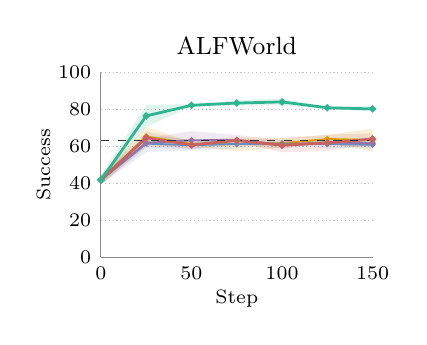
\begin{tikzpicture}
\begin{axis}[
  width=3.45cm, height=2.35cm, scale only axis, xmin=0, xmax=150, ymin=0, ymax=100, xtick={0,50,100,150},
  axis lines*=left, axis line style={black!45}, tick style={draw=none}, ytick pos=left,
  ymajorgrids, grid style={densely dotted, black!25}, every tick label/.append style={font=\scriptsize},
  xlabel={Step}, xlabel style={font=\scriptsize, yshift=3pt}, ylabel={Success}, ylabel style={font=\scriptsize, yshift=-4pt},
  title={ALFWorld}, title style={font=\small, yshift=-3pt},
]
\addplot[fill=cTcod, fill opacity=0.15, draw=none, forget plot] coordinates {(0,44.26) (25,70.60) (50,62.35) (75,65.18) (100,64.30) (125,66.16) (150,69.60) (150,57.15) (125,61.70) (100,58.99) (75,57.29) (50,59.95) (25,60.00) (0,39.37)} \closedcycle;
\addplot[fill=cGuided, fill opacity=0.15, draw=none, forget plot] coordinates {(0,44.26) (25,66.00) (50,63.53) (75,63.69) (100,61.74) (125,63.55) (150,62.12) (150,59.60) (125,58.81) (100,61.19) (75,58.82) (50,57.69) (25,56.89) (0,39.37)} \closedcycle;
\addplot[fill=cFtb, fill opacity=0.15, draw=none, forget plot] coordinates {(0,44.26) (25,64.34) (50,68.17) (75,66.15) (100,63.03) (125,62.35) (150,65.00) (150,58.40) (125,61.73) (100,58.66) (75,60.58) (50,58.34) (25,59.38) (0,39.37)} \closedcycle;
\addplot[fill=vanRed, fill opacity=0.15, draw=none, forget plot] coordinates {(0,44.26) (25,67.85) (50,62.90) (75,63.80) (100,64.39) (125,66.27) (150,67.03) (150,60.82) (125,57.45) (100,56.75) (75,62.51) (50,58.53) (25,61.39) (0,39.37)} \closedcycle;
\addplot[fill=r2sGreen, fill opacity=0.15, draw=none, forget plot] coordinates {(0,44.26) (25,82.25) (50,82.87) (75,84.83) (100,85.67) (125,81.54) (150,81.65) (150,78.78) (125,80.07) (100,82.29) (75,81.89) (50,81.43) (25,70.57) (0,39.37)} \closedcycle;
\addplot[cTcod, line width=0.7pt, mark=*, mark size=0.7pt] coordinates {(0,41.82) (25,65.30) (50,61.15) (75,61.23) (100,61.65) (125,63.93) (150,63.38)};
\addplot[cGuided, line width=0.7pt, mark=*, mark size=0.7pt] coordinates {(0,41.82) (25,61.44) (50,60.61) (75,61.26) (100,61.46) (125,61.18) (150,60.86)};
\addplot[cFtb, line width=0.7pt, mark=*, mark size=0.7pt] coordinates {(0,41.82) (25,61.86) (50,63.25) (75,63.37) (100,60.85) (125,62.04) (150,61.70)};
\addplot[vanRed, line width=1.0pt, mark=*, mark size=0.7pt] coordinates {(0,41.82) (25,64.62) (50,60.72) (75,63.16) (100,60.57) (125,61.86) (150,63.92)};
\addplot[r2sGreen, line width=1.0pt, mark=*, mark size=0.7pt] coordinates {(0,41.82) (25,76.41) (50,82.15) (75,83.36) (100,83.98) (125,80.81) (150,80.21)};
\draw[dashed, black!80, line width=0.6pt] (axis cs:0,63.08) -- (axis cs:150,63.08);
\end{axis}
\end{tikzpicture}
\hfill
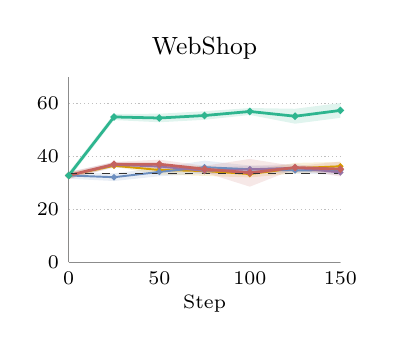
\begin{tikzpicture}
\begin{axis}[
  width=3.45cm, height=2.35cm, scale only axis, xmin=0, xmax=150, ymin=0, ymax=70, xtick={0,50,100,150},
  axis lines*=left, axis line style={black!45}, tick style={draw=none}, ytick pos=left,
  ymajorgrids, grid style={densely dotted, black!25}, every tick label/.append style={font=\scriptsize},
  xlabel={Step}, xlabel style={font=\scriptsize, yshift=3pt}, ylabel={}, ylabel style={font=\scriptsize, yshift=-4pt},
  title={WebShop}, title style={font=\small, yshift=-3pt},
]
\addplot[fill=cTcod, fill opacity=0.15, draw=none, forget plot] coordinates {(0,34.05) (25,36.88) (50,36.57) (75,36.31) (100,34.62) (125,37.54) (150,37.93) (150,34.60) (125,33.53) (100,32.05) (75,32.62) (50,33.17) (25,36.05) (0,31.55)} \closedcycle;
\addplot[fill=cGuided, fill opacity=0.15, draw=none, forget plot] coordinates {(0,34.05) (25,33.58) (50,35.76) (75,38.40) (100,36.55) (125,35.91) (150,36.54) (150,33.06) (125,33.56) (100,33.71) (75,33.46) (50,32.50) (25,30.69) (0,31.55)} \closedcycle;
\addplot[fill=cFtb, fill opacity=0.15, draw=none, forget plot] coordinates {(0,34.05) (25,37.86) (50,37.00) (75,35.69) (100,36.46) (125,37.17) (150,34.44) (150,33.43) (125,34.17) (100,33.80) (75,33.38) (50,35.40) (25,35.74) (0,31.55)} \closedcycle;
\addplot[fill=vanRed, fill opacity=0.15, draw=none, forget plot] coordinates {(0,34.05) (25,37.92) (50,38.77) (75,36.45) (100,39.04) (125,36.33) (150,38.02) (150,32.38) (125,35.27) (100,28.56) (75,33.95) (50,35.37) (25,36.08) (0,31.55)} \closedcycle;
\addplot[fill=r2sGreen, fill opacity=0.15, draw=none, forget plot] coordinates {(0,34.05) (25,56.11) (50,56.15) (75,57.08) (100,58.31) (125,58.02) (150,60.20) (150,54.60) (125,52.38) (100,55.69) (75,53.85) (50,52.92) (25,53.76) (0,31.55)} \closedcycle;
\addplot[cTcod, line width=0.7pt, mark=*, mark size=0.7pt] coordinates {(0,32.80) (25,36.47) (50,34.87) (75,34.47) (100,33.33) (125,35.53) (150,36.27)};
\addplot[cGuided, line width=0.7pt, mark=*, mark size=0.7pt] coordinates {(0,32.80) (25,32.13) (50,34.13) (75,35.93) (100,35.13) (125,34.73) (150,34.80)};
\addplot[cFtb, line width=0.7pt, mark=*, mark size=0.7pt] coordinates {(0,32.80) (25,36.80) (50,36.20) (75,34.53) (100,35.13) (125,35.67) (150,33.93)};
\addplot[vanRed, line width=1.0pt, mark=*, mark size=0.7pt] coordinates {(0,32.80) (25,37.00) (50,37.07) (75,35.20) (100,33.80) (125,35.80) (150,35.20)};
\addplot[r2sGreen, line width=1.0pt, mark=*, mark size=0.7pt] coordinates {(0,32.80) (25,54.93) (50,54.53) (75,55.47) (100,57.00) (125,55.20) (150,57.40)};
\draw[dashed, black!80, line width=0.6pt] (axis cs:0,33.53) -- (axis cs:150,33.53);
\end{axis}
\end{tikzpicture}
\hfill
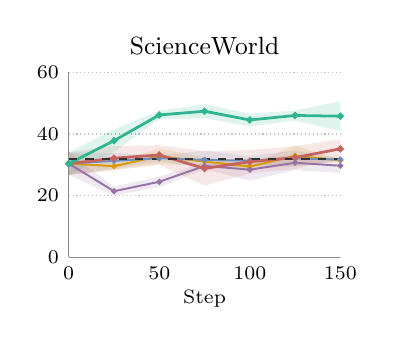
\begin{tikzpicture}
\begin{axis}[
  width=3.45cm, height=2.35cm, scale only axis, xmin=0, xmax=150, ymin=0, ymax=60, xtick={0,50,100,150},
  axis lines*=left, axis line style={black!45}, tick style={draw=none}, ytick pos=left,
  ymajorgrids, grid style={densely dotted, black!25}, every tick label/.append style={font=\scriptsize},
  xlabel={Step}, xlabel style={font=\scriptsize, yshift=3pt}, ylabel={}, ylabel style={font=\scriptsize, yshift=-4pt},
  title={ScienceWorld}, title style={font=\small, yshift=-3pt},
]
\addplot[fill=cTcod, fill opacity=0.15, draw=none, forget plot] coordinates {(0,34.07) (25,30.58) (50,35.31) (75,32.40) (100,30.15) (125,36.23) (150,31.92) (150,31.00) (125,29.56) (100,28.70) (75,29.70) (50,30.24) (25,28.53) (0,26.68)} \closedcycle;
\addplot[fill=cGuided, fill opacity=0.15, draw=none, forget plot] coordinates {(0,34.07) (25,33.78) (50,33.06) (75,34.58) (100,32.87) (125,34.65) (150,32.01) (150,31.41) (125,29.51) (100,29.79) (75,28.66) (50,31.17) (25,28.78) (0,26.68)} \closedcycle;
\addplot[fill=cFtb, fill opacity=0.15, draw=none, forget plot] coordinates {(0,34.07) (25,22.89) (50,26.19) (75,30.73) (100,32.00) (125,33.05) (150,32.07) (150,27.31) (125,28.25) (100,24.86) (75,28.51) (50,22.78) (25,19.99) (0,26.68)} \closedcycle;
\addplot[fill=vanRed, fill opacity=0.15, draw=none, forget plot] coordinates {(0,34.07) (25,36.11) (50,36.36) (75,34.38) (100,34.78) (125,36.07) (150,38.31) (150,32.07) (125,28.58) (100,27.21) (75,23.24) (50,30.01) (25,28.18) (0,26.68)} \closedcycle;
\addplot[fill=r2sGreen, fill opacity=0.15, draw=none, forget plot] coordinates {(0,34.07) (25,41.55) (50,47.55) (75,49.63) (100,46.60) (125,47.62) (150,50.57) (150,40.94) (125,44.36) (100,42.46) (75,45.08) (50,44.77) (25,34.09) (0,26.68)} \closedcycle;
\addplot[cTcod, line width=0.7pt, mark=*, mark size=0.7pt] coordinates {(0,30.37) (25,29.55) (50,32.77) (75,31.05) (100,29.42) (125,32.90) (150,31.46)};
\addplot[cGuided, line width=0.7pt, mark=*, mark size=0.7pt] coordinates {(0,30.37) (25,31.28) (50,32.12) (75,31.62) (100,31.33) (125,32.08) (150,31.71)};
\addplot[cFtb, line width=0.7pt, mark=*, mark size=0.7pt] coordinates {(0,30.37) (25,21.44) (50,24.49) (75,29.62) (100,28.43) (125,30.65) (150,29.69)};
\addplot[vanRed, line width=1.0pt, mark=*, mark size=0.7pt] coordinates {(0,30.37) (25,32.14) (50,33.18) (75,28.81) (100,31.00) (125,32.33) (150,35.19)};
\addplot[r2sGreen, line width=1.0pt, mark=*, mark size=0.7pt] coordinates {(0,30.37) (25,37.82) (50,46.16) (75,47.36) (100,44.53) (125,45.99) (150,45.76)};
\draw[dashed, black!80, line width=0.6pt] (axis cs:0,31.96) -- (axis cs:150,31.96);
\end{axis}
\end{tikzpicture}
\\[2pt]
{\scriptsize \tikz[baseline=-0.4ex]{\draw[vanRed, line width=0.9pt] (0,0.065) -- (0.4,0.065);}\,Vanilla OPD\quad\tikz[baseline=-0.4ex]{\draw[cTcod, line width=0.9pt] (0,0.065) -- (0.4,0.065);}\,TCOD-F2B\quad\tikz[baseline=-0.4ex]{\draw[cGuided, line width=0.9pt] (0,0.065) -- (0.4,0.065);}\,Guided-OPD\quad\tikz[baseline=-0.4ex]{\draw[cFtb, line width=0.9pt] (0,0.065) -- (0.4,0.065);}\,FutureBridge\quad\tikz[baseline=-0.4ex]{\draw[r2sGreen, line width=0.9pt] (0,0.065) -- (0.4,0.065);}\,\method{}\quad\tikz[baseline=-0.4ex]{\draw[dashed, black!80, line width=0.6pt] (0,0.065) -- (0.4,0.065);}\,Teacher Alone}
\caption{\textbf{\method{} students separate from every baseline during training.} Qwen3.5-9B teaches Qwen3.5-4B; mean $\pm$ one standard deviation over three training runs; dashed: the teacher acting alone. Other teacher--student pairs are in \Cref{app:curves}.}
\label{fig:teacher-bars}\label{fig:curves}
\end{figure}


\textbf{\method{} beats every baseline in all twelve cells of \Cref{tab:main} and ends above the teacher acting alone.} The gain over vanilla OPD averages $+17.8$ points from the 9B teacher and $+9.8$ from the 30B-A3B teacher, and \method{} exceeds every baseline in mean on all $24$ splits of \Cref{tab:main-full}.
Averaged over the ten cells outside the 30B-A3B teacher's WebShop pair, the vanilla student ends within a point of the teacher acting alone. On WebShop the 30B-A3B teacher acting alone seldom completes a purchase: on $13.7$ of its $15$ turns per episode, on average, it answers without calling the action tool, so $94\%$ of its episodes run out of turns, and every student ends above it. \Cref{fig:teacher-bars} follows the Qwen3.5-9B-to-4B students of all five methods over three training runs each: the \method{} student separates from every baseline well before the final checkpoint. The three \method{} runs share the one repaired teacher of \Cref{tab:main}, so the width of its band comes from student training alone. The teacher's takeovers from the untrained student's highest-disagreement states finish more often than the student does in eleven of the twelve cells (\Cref{tab:takeover-all} in \Cref{app:analysis}), so what \Cref{sec:takeover} found for one pair holds for all four.

\begin{table}[h]
\centering
\caption{\textbf{Self-distillation: Qwen3.5-4B teaches Qwen3.5-4B.} \method{} first repairs the 4B teacher on its own takeovers; the other arms learn from the unrepaired 4B.}
\label{tab:self}
\small
\setlength{\tabcolsep}{4.5pt}
\begin{tabular}{@{}lcccccc@{}}
\toprule
Environment & Student alone & Vanilla OPD & TCOD-F2B & Guided-OPD & FutureBridge & \textbf{\textcolor{box_green}{\method{} (ours)}} \\
\midrule\midrule
ALFWorld & $43.4{\pm}1.0$ & $49.9{\pm}2.6$ & $49.7{\pm}2.6$ & $48.5{\pm}3.8$ & \secondscore{$50.6{\pm}1.9$} & \bestscore{$72.7{\pm}1.3$} \\
WebShop & $33.7{\pm}0.9$ & $33.3{\pm}2.2$ & $31.3{\pm}0.9$ & \secondscore{$34.0{\pm}1.8$} & $31.1{\pm}1.5$ & \bestscore{$58.1{\pm}2.5$} \\
ScienceWorld & $28.0{\pm}1.5$ & $28.2{\pm}2.3$ & $27.2{\pm}0.8$ & \secondscore{$29.3{\pm}1.8$} & $29.2{\pm}2.9$ & \bestscore{$42.4{\pm}3.4$} \\
\bottomrule
\end{tabular}
\end{table}


\textbf{The teacher can be the student's own base model.}
\Cref{tab:self} repeats the Qwen3.5-4B cells with the 4B as its own teacher. In all three environments, the \method{} student taught by the repaired 4B passes the vanilla student that the 9B teaches in \Cref{tab:main}. Since the teacher and the student are the same model, the student--teacher gap that ranks states is zero, so the pipeline draws one turn per episode of the untrained student at random under the same goal cap and budget; the 4B itself runs the takeovers and the selection, so no larger model enters the pipeline. In all three environments this self-taught student also ends above the 9B teacher acting alone in \Cref{tab:main}. Taught by the unrepaired 4B, the four other students gain about six points on ALFWorld and at most about a point on WebShop and ScienceWorld: a model's plain scores of its own tokens teach it little. What lifts the student is not a larger model's knowledge but scores informed by the ending, which its own base model can supply.

\Needspace{17\baselineskip}
\subsection{Ablations}
\label{sec:exp-repair}

\begin{wraptable}{r}{0.5\textwidth}
\vspace{-10pt}
\centering
\caption{\raggedright Ablation on \textbf{takeover selection}. Success (\%). Ground truth reads the task reward and is not ranked.}
\label{tab:selection}
\fontsize{8}{9.5}\selectfont
\setlength{\tabcolsep}{4pt}
\begin{tabular}{@{}lccc@{}}
\toprule
& \textbf{ALFWorld} & \textbf{WebShop} & \textbf{ScienceWorld} \\
\midrule\midrule
Vanilla OPD & $65.8{\pm}2.6$ & $34.6{\pm}2.9$ & $34.6{\pm}3.5$ \\
Consensus vote & \secondscore{$81.9{\pm}2.4$} & \bestscore{$63.1{\pm}1.6$} & \secondscore{$39.5{\pm}2.9$} \\
LLM judge & \bestscore{$82.6{\pm}0.9$} & \secondscore{$55.9{\pm}1.4$} & \bestscore{$50.3{\pm}1.5$} \\
\midrule
Ground truth & $85.9{\pm}1.2$ & $65.0{\pm}1.4$ & $49.0{\pm}1.1$ \\
\bottomrule
\end{tabular}
\vspace{-9pt}
\end{wraptable}

Each ablation below varies one part of \method{} in the Qwen3.5-9B-to-4B cells of \Cref{tab:main}, on all three environments.

\textbf{Takeover selection.}\label{sec:exp-select}
\Cref{tab:selection} repairs the teacher with three rules for picking the winning takeovers. Ground truth reads the task reward; the consensus vote and the LLM judge do not. With either reward-free rule the student ends above vanilla OPD in all three environments, so the repair depends neither on reading the reward nor on one particular rule.

\Needspace{14\baselineskip}
\begin{wraptable}{r}{0.55\textwidth}
\vspace{-10pt}
\centering
\caption{\raggedright Ablation on \textbf{components}. Success (\%); the rows are vanilla OPD, label-SFT and \method{}.}
\label{tab:abl-components}
\fontsize{8}{9.5}\selectfont
\setlength{\tabcolsep}{3pt}
\begin{tabular}{@{}cc|ccc@{}}
\toprule
\textbf{Takeovers} & \shortstack{\textbf{Informed}\\\textbf{targets}} & \textbf{ALFWorld} & \textbf{WebShop} & \textbf{ScienceWorld} \\
\midrule\midrule
\textcolor{gray}{\xmark} & \textcolor{gray}{\xmark} & $65.8{\pm}2.6$ & $34.6{\pm}2.9$ & $34.6{\pm}3.5$ \\
\textcolor{box_green}{\cmark} & \textcolor{gray}{\xmark} & \secondscore{$76.8{\pm}3.5$} & \secondscore{$46.7{\pm}1.3$} & \secondscore{$41.0{\pm}3.0$} \\
\midrule
\textcolor{box_green}{\cmark} & \textcolor{box_green}{\cmark} & \bestscore{$81.9{\pm}2.4$} & \bestscore{$55.9{\pm}1.4$} & \bestscore{$47.8{\pm}3.0$} \\
\bottomrule
\end{tabular}
\vspace{-8pt}
\end{wraptable}


\textbf{Effect of informed targets.}
\Cref{tab:abl-components} separates the takeovers from the informed targets built on them. The label-SFT control fine-tunes the teacher on the selected takeovers by standard SFT. Its student already ends well above vanilla OPD in all three environments, so the takeovers carry signal of their own; fitting the informed targets instead lifts the student further. The takeovers help most as context for the teacher's scores of the student's own tokens, not as SFT data.

\Needspace{13\baselineskip}
\begin{wraptable}{r}{0.55\textwidth}
\vspace{-10pt}
\centering
\caption{\raggedright Ablation on \textbf{supervised turns}. Success (\%); the suffix, from the divergence turn to the end, is \method{}.}
\label{tab:abl-scope}
\fontsize{8}{9.5}\selectfont
\setlength{\tabcolsep}{3pt}
\begin{tabular}{@{}lcccc@{}}
\toprule
& \textbf{ALFWorld} & \textbf{WebShop} & \textbf{ScienceWorld} & \textbf{Avg.} \\
\midrule\midrule
Divergence turn & \bestscore{$82.5{\pm}2.3$} & $48.5{\pm}1.4$ & \bestscore{$48.7{\pm}0.4$} & 59.9 \\
Prefix & $81.0{\pm}1.8$ & \secondscore{$52.7{\pm}0.8$} & $47.6{\pm}2.1$ & \secondscore{60.5} \\
Suffix & \secondscore{$81.9{\pm}2.4$} & \bestscore{$55.9{\pm}1.4$} & \secondscore{$47.8{\pm}3.0$} & \bestscore{61.9} \\
\bottomrule
\end{tabular}
\end{wraptable}

\textbf{Supervised turns.}
\method{} fits the informed targets on the suffix of the student's episode, from the divergence turn to its end. \Cref{tab:abl-scope} supervises instead the divergence turn alone or the prefix up to it. Every span lifts the student well above vanilla OPD in all three environments, so the informed targets help whichever turns they cover. Vanilla OPD, whose teacher scores each token without seeing how the episode ends, trails them all by a wide margin.

\subsection{Long-Horizon Behavior}
\label{sec:exp-longhorizon}

We compare the Qwen3.5-9B-to-4B \method{} teachers and students of \Cref{tab:main} with vanilla OPD.

\begin{figure}[t]
\centering
\definecolor{vanRed}{HTML}{C5635F}
\definecolor{r2sGreen}{HTML}{2EB58F}
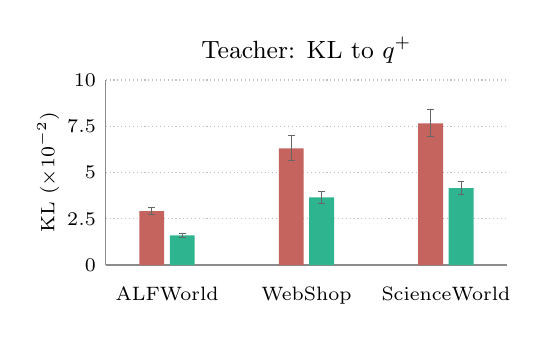
\begin{tikzpicture}
\begin{axis}[
  width=5.1cm, height=2.35cm, scale only axis, ybar, bar width=9pt, bar shift auto, enlarge x limits=0.22,
  symbolic x coords={ALFWorld,WebShop,ScienceWorld}, xtick=data, ymin=0, ymax=10, ytick={0,2.5,5,7.5,10},
  axis lines*=left, axis line style={black!45}, tick style={draw=none}, ytick pos=left,
  ymajorgrids, grid style={densely dotted, black!25}, every tick label/.append style={font=\scriptsize},
  ylabel={KL ($\times 10^{-2}$)}, ylabel style={font=\scriptsize, yshift=-4pt},
  title={Teacher: KL to $q^{+}$}, title style={font=\small, yshift=-3pt, text height=1.8ex, text depth=0.3ex},
  error bars/y dir=both, error bars/y explicit, error bars/error bar style={black!60, line width=0.4pt},
  error bars/error mark options={rotate=90, black!60, mark size=1.2pt},
]
\addplot[fill=vanRed, draw=none] coordinates {(ALFWorld,2.91) += (0,0.22) -= (0,0.20) (WebShop,6.31) += (0,0.67) -= (0,0.67) (ScienceWorld,7.66) += (0,0.74) -= (0,0.69)};
\addplot[fill=r2sGreen, draw=none] coordinates {(ALFWorld,1.60) += (0,0.10) -= (0,0.10) (WebShop,3.65) += (0,0.33) -= (0,0.32) (ScienceWorld,4.15) += (0,0.36) -= (0,0.34)};
\end{axis}
\end{tikzpicture}
\hfill
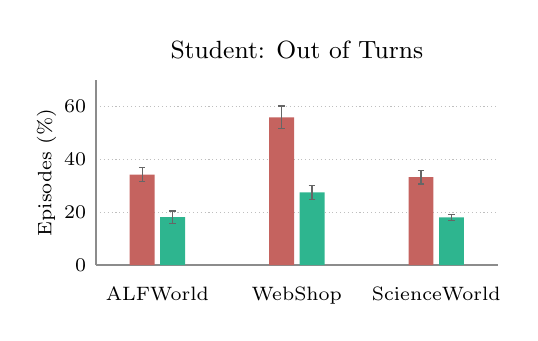
\begin{tikzpicture}
\begin{axis}[
  width=5.1cm, height=2.35cm, scale only axis, ybar, bar width=9pt, bar shift auto, enlarge x limits=0.22,
  symbolic x coords={ALFWorld,WebShop,ScienceWorld}, xtick=data, ymin=0, ymax=70, ytick={0,20,40,60},
  axis lines*=left, axis line style={black!45}, tick style={draw=none}, ytick pos=left,
  ymajorgrids, grid style={densely dotted, black!25}, every tick label/.append style={font=\scriptsize},
  ylabel={Episodes (\%)}, ylabel style={font=\scriptsize, yshift=-4pt},
  title={Student: Out of Turns}, title style={font=\small, yshift=-3pt, text height=1.8ex, text depth=0.3ex},
  error bars/y dir=both, error bars/y explicit, error bars/error bar style={black!60, line width=0.4pt},
  error bars/error mark options={rotate=90, black!60, mark size=1.2pt},
]
\addplot[fill=vanRed, draw=none] coordinates {(ALFWorld,34.18) +- (0,2.65) (WebShop,55.87) +- (0,4.28) (ScienceWorld,33.24) +- (0,2.59)};
\addplot[fill=r2sGreen, draw=none] coordinates {(ALFWorld,18.10) +- (0,2.36) (WebShop,27.53) +- (0,2.66) (ScienceWorld,18.02) +- (0,1.13)};
\end{axis}
\end{tikzpicture}

{\scriptsize \tikz[baseline=-0.4ex]{\fill[vanRed] (0,-0.02) rectangle (0.3,0.16);}\,Vanilla OPD\quad\tikz[baseline=-0.4ex]{\fill[r2sGreen] (0,-0.02) rectangle (0.3,0.16);}\,\method{}}
\caption{\textbf{Repair moves the teacher toward its informed targets, and its student runs out of turns about half as often.} Left: each teacher's top-16 KL to $q^{+}$ on held-out states, with 95\% goal-bootstrap intervals. Right: held-out episodes that end unfinished at the turn budget, mean $\pm$ std over three decodes.}
\label{fig:scorer-effect}
\end{figure}


\textbf{Repair brings the teacher closer to its informed targets, and its student runs out of turns less often.} Scored against the same $q^{+}$ targets over the complete assistant suffix of held-out states, the repaired teacher is closer to them than the unrepaired teacher in every environment, as the left panel of \Cref{fig:scorer-effect} shows. In the evaluation episodes behind \Cref{tab:main}, the student trained on the repaired teacher runs out of turns about half as often as the vanilla OPD student, as the right panel shows.

\begin{table}[t]
\centering
\caption{\textbf{The vanilla student inherits the teacher's endings; the repaired student does not.} Held-out episodes that run out of turns (\%) and turns per episode, seen split, over three decodes.}
\label{tab:timeouts}
\small
\setlength{\tabcolsep}{4pt}
\begin{tabular}{@{}lcccccc@{}}
\toprule
\multirow{2}{*}{Method} & \multicolumn{2}{c}{ALFWorld} & \multicolumn{2}{c}{WebShop} & \multicolumn{2}{c}{ScienceWorld} \\
\cmidrule(lr){2-3}\cmidrule(lr){4-5}\cmidrule(l){6-7}
 & Out of turns & Turns & Out of turns & Turns & Out of turns & Turns \\
\midrule\midrule
Teacher alone & $39.8{\pm}1.5$ & $20.0$ & $56.7{\pm}0.9$ & $11.9$ & $35.7{\pm}1.9$ & $19.7$ \\
Student alone & $55.0{\pm}3.6$ & $22.3$ & $56.7{\pm}1.2$ & $11.9$ & $38.6{\pm}2.1$ & $17.7$ \\
\midrule
Vanilla OPD & \secondscore{$34.3{\pm}4.7$} & \secondscore{$19.0$} & \secondscore{$55.9{\pm}4.3$} & \secondscore{$11.8$} & \secondscore{$31.9{\pm}1.5$} & \secondscore{$18.9$} \\
\textbf{\textcolor{box_green}{\method{} (ours)}} & \bestscore{$19.5{\pm}2.2$} & \bestscore{$14.7$} & \bestscore{$27.5{\pm}2.7$} & \bestscore{$9.0$} & \bestscore{$17.1{\pm}0.7$} & \bestscore{$14.5$} \\
\bottomrule
\end{tabular}
\end{table}


\textbf{The vanilla student inherits the teacher's endings.} \Cref{tab:timeouts} counts, for the same evaluation episodes, how often each policy runs out of turns and how many turns it takes, beside the teacher acting alone and the untrained student. On ALFWorld every failure is a timeout, since the wrapper ends an episode only on success. In every environment the vanilla student takes about the teacher's number of turns and runs out of turns almost as often as the teacher does. The \method{} student finishes in fewer turns and runs out of turns far less often than the teacher that scores it.

\textbf{The saved turns are searching turns.} \Cref{tab:search-turns} splits the turns of the students' training rollouts into searching, that is moving, opening and looking, or searching and paging on WebShop, and acting on the task. The \method{} student spends fewer turns searching than the vanilla OPD student in every environment and about as many on the task. Counting only the episodes each student wins, it still searches less: $8.4$ turns against $10.5$ on ALFWorld, $2.0$ against $3.0$ on WebShop and $7.1$ against $9.1$ on ScienceWorld. On ALFWorld it opens fewer receptacles, on ScienceWorld it looks, reads and waits less, and on WebShop it searches and pages less and buys more. This matches the direction of the informed scores in \Cref{tab:drift}, which fall most on the student's hedging and searching words.

\begin{table}[h]
\centering
\caption{\textbf{The repaired student spends fewer turns searching.} Turns per episode in the last ten training updates, mean$\pm$std over three training runs. \emph{Task} turns act on the goal, such as taking or buying.}
\label{tab:search-turns}
\vspace{2pt}
\small
\setlength{\tabcolsep}{2.5pt}
\begin{tabular}{@{}lccccccccc@{}}
\toprule
\multirow{2}{*}{Method} & \multicolumn{3}{c}{ALFWorld} & \multicolumn{3}{c}{WebShop} & \multicolumn{3}{c}{ScienceWorld} \\
\cmidrule(lr){2-4}\cmidrule(lr){5-7}\cmidrule(l){8-10}
 & Turns & Searching & Task & Turns & Searching & Task & Turns & Searching & Task \\
\midrule\midrule
Vanilla OPD & \secondscore{$20.7{\pm}0.9$} & \secondscore{$15.9{\pm}1.2$} & \secondscore{$4.0{\pm}0.3$} & \secondscore{$11.5{\pm}0.4$} & \secondscore{$7.8{\pm}0.5$} & \secondscore{$3.6{\pm}0.1$} & \secondscore{$18.2{\pm}0.5$} & \secondscore{$10.9{\pm}0.6$} & \secondscore{$6.9{\pm}0.7$} \\
\method{} & \bestscore{$15.6{\pm}0.5$} & \bestscore{$11.4{\pm}0.6$} & \bestscore{$3.7{\pm}0.3$} & \bestscore{$8.8{\pm}0.2$} & \bestscore{$4.1{\pm}0.1$} & \bestscore{$4.7{\pm}0.1$} & \bestscore{$14.6{\pm}0.3$} & \bestscore{$8.2{\pm}0.6$} & \bestscore{$6.1{\pm}0.3$} \\
\bottomrule
\end{tabular}
\end{table}

